\section{Технические характеристики линий передаич данных} %9

\subsection{Описание адаптированного IPv6 уровня} %9.4
 
\subsubsection{Ввод в эксплуатацию новых устройств} %9.4.4

Расширение к приложению Е % 9.4.4.2

Формат сообщений протокола начальной загрузки LoWPAN (LBP) % 9.4.4.2.1

Описание % 9.4.4.2.1.1 

Формат LBP сообшений и детали их содержимого описаны на рисунке \ref{img:9-22} и в таблице 2. % \ref{tab:9-46} 

\begin{figure}[h]
 \label{img:9-22}
 \center{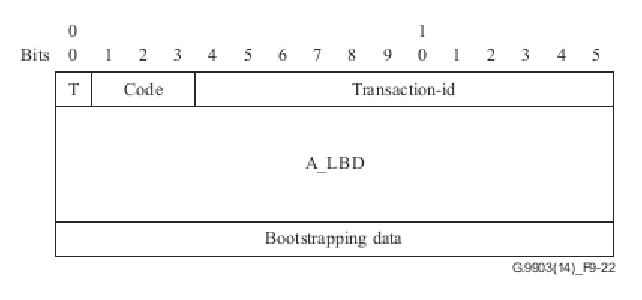
\includegraphics{pictures/9-22}}
 \caption{формат LBP сообщения}
\end{figure}

\begin{longtable}[\textwidth]{|p{0.2\linewidth}|p{0.15\linewidth}|p{0.65\linewidth}|}
\caption{формат LBP сообщения} \\ % \ref{tab:9-46}
\hline
Поле & Размер & Описание \\ \hline
Т & 1 бит & Определяет тип сообщения: \\
& & 0: Сообщение от LBD \\
& & 1: Сообщение для LBD \\ \hline
Код & 3 бита & Определяет код сообщения. Подробности в таблице 9-47 \\ \hline
ID транзакции & 12 бит & Зарезервированно ITU-T. Устанавливается значение 0 при отправлении. При получении игнорируется \\ \hline
A\_LBD & 8 байт & Указывает EUI-64 адрес устройства(LBD)  при автозагрузке\\ \hline
Данные автонастройки & переменная длина & Содержит дополнительнеы информационные элементы. Бывает двух типов: \\
& & Встроенные EAP-сообщения (пункт 9.4.4.2.1.2) \\
& & Параметры настройки (пункт 9.4.4.2.1.3) \\ \hline
\end{longtable}

\begin{longtable}[\textwidth]{|p{0.05\textwidth}|p{0.1\textwidth}|p{0.2\textwidth}|p{0.65\textwidth}|}
\caption{значение полей Т и Код в LBP-сообщении} \\ % \ref{tab:9-47}
\hline
Т & Код & LBP-сообщение & Описание \\ \hline
0 & 0b001 & JOINING & LBD запрос. Передает в себе PAN и материалы, необходимые для аутентификации. \\ \hline
1 & 0b001 & ACCEPTED & Ответ LBD об успешной аутентификации. Несет в себе спецификацию устройства(DSI) \\ \hline
1 & 0b010 & CHALLENGE & Идет аутентификация. Может передавать на LBD спецификацию PAN (PSI) \\ \hline
1 & 0b011 & DECLINE & Аутентификация провалена \\ \hline
0/1 & 0b100 & KICK & Испольуется координатором PAN для того, что бы устройство потеряло свой MAC-адрес. Или наоборот использоваться устройсвтом для инфомрирования PAN о потере MAC-адреса. При получении данного кадра устройство должно выставить свой адрес на стандартное значение 0xFFFF, отключить себя от сети и выполнить сбор MAC и уровня адаптации. Подробнее процедура KICK описана в пункте 9.4.4.2.2.7 \\ \hline
\end{longtable}

Встроенные сообщения EAP % 9.4.4.2.1.2

LBM сообщения вкладывают особые аутентификационные сообщения (EAP) описанные в IETF RFC 3748. На рисунке \ref{img:9-23} представлены изменения, необходимые для соответствия информационным LBP элементам. В таблице 1 описаны поля сообщения.  %\ref{tab:9-48}

\begin{figure}[h]
 \label{img:9-23}
 \center{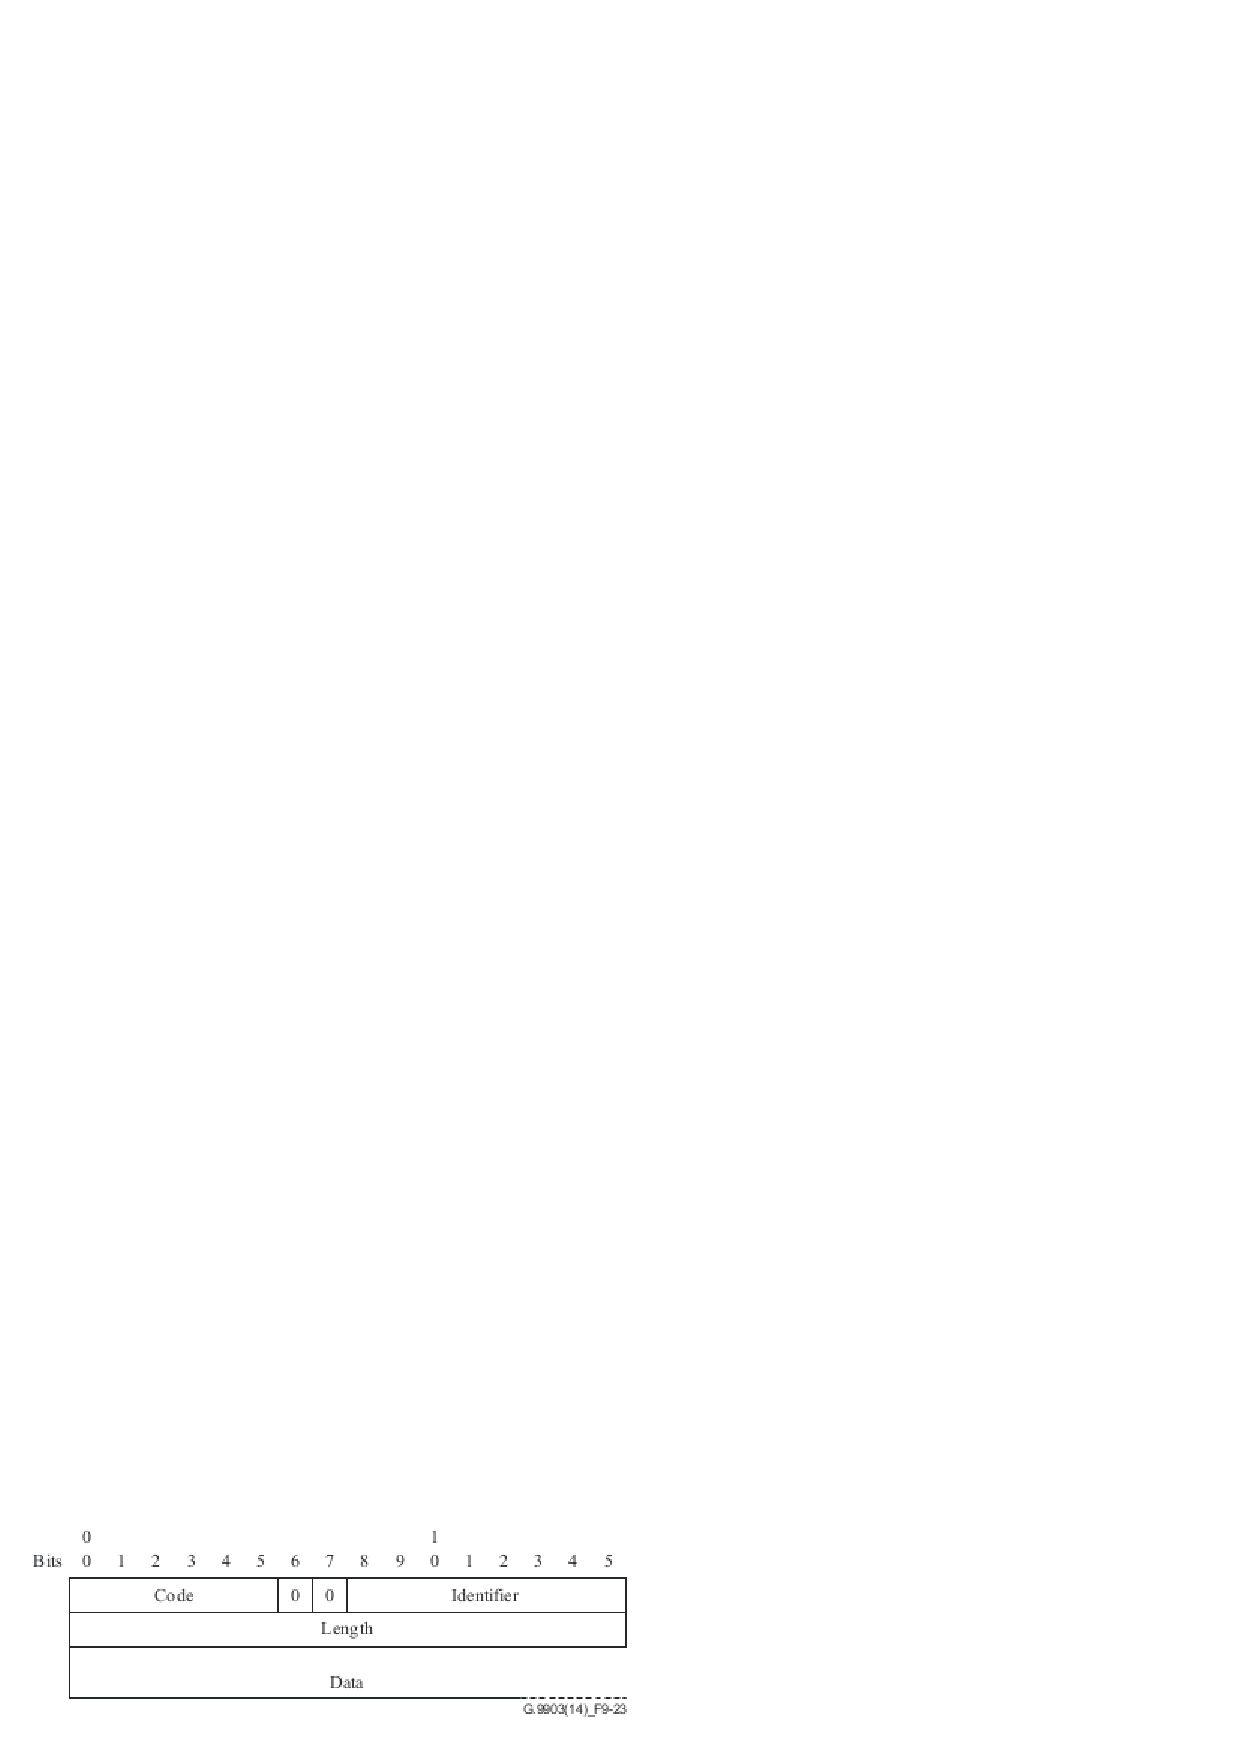
\includegraphics{pictures/9-23}}
 \caption{Общий формат EAP сообшения}
\end{figure}

\begin{longtable}[\textwidth]{|p{0.21\linewidth}|p{0.15\linewidth}|p{0.64\linewidth}|}
\caption{Поля, встроенные в EAP сообшение} \\ % \ref{tab:9-48}
\hline
Поле & Размер & Описание \\ \hline
Код & 6 бит & Определяет тип EAP покета. Каждый код соответствует: \\
& & 0b000001: Запрос (клиентк отправлен LBP) \\
& & 0b000010: Ответ (получен от клиента) \\
& & 0b000011: Успех (отправления клиенту) \\
& & 0b000100: Неудача (отправления клиенту) \\
& & Поле кода отличается от стандартного поля кода EAP. Существует простое двустороннее преобразование описанное в IETF RFC 3748. Преобразование провизводится если происходит передача покета по другому протоколу (например RADIUS) и в случае контроля целостности EAP заголовка. \\ \hline
Идентификатор &  8 бит & Помогает при согласовании ответа с запросом. \\ \hline
Длина & 16 бит & Указывает размер пакета в байтах. Включает в себя поле кода, идентификатора, длины и поля данных. Сообщения, с длиной, меньше указанной в поле, должны игнорироваться. \\ \hline
Данные & переменная длина & Формат поля данных опрелеляется полем кода. Больше информации в IETF RFC 3748 \\ \hline
\end{longtable}
